%% JPEG Preimage %%%%%%%%%%%%%%%%%%%%%%%%%%%%%%%%%%%%%%%%%%%%%%%%%%%%%%%
\section{JPEG Preimage}
\label{sec:jpeg}

%\newcommand{\Int}[0]{\mathrm{Z}}

To validate our work, we have applied BLT to the problem of
computing preimages from JPEG decompression.

To simplify exposition, we will restrict our attention to
\emph{monochrome} JPEG images that consist of a single
$8\times{}8$ block of pixels.
%
In experiments, we have also applied BLT to color images; color
problems involve more variables and constraints, but are otherwise similar
to the monochrome case.
%
Our restriction to images that are $8$ by $8$ does not effect
scalability either; JPEG compresses each $8\times{}8$ block of
pixels within an image independently, so computing the preimage
for a larger image is the same as finding preimages for multiple
independent $8$ by $8$ blocks.

When compressing an image, each pixel ranges from
$0$ to $255$ where $0$ corresponds to black and $255$ corresponds to white.
To compress an image, JPEG performs the following steps~\cite{jpeg}:

\newcommand{\dct}{\mathrm{dct}_2}
\newcommand{\idct}{\mathrm{idct}_2}

\begin{enumerate}

\item Each pixel value is shifted by $-128$ so that the pixel
   values range between $-128$ and $127$.

\item A 2d discrete cosine transform (DCT) is applied to each block
    that transforms the coordinate space from the image pixel values to
    the frequency domain.  This has the effect of separating out the
    image components by frequency, so that course grained qualities
    such as overall brightness are represented distinctly from more
    fine-grained fluctuations.  For a given input block
    $I$, we denote the frequency representation by $F = \dct(I)$.
    A 2d DCT is obtained by first applying a 1d DCT to each
    column in the image, and then applying a 1d DCT to each row
    in the image.

\item A quantization step is performed in which each coordinate in
    the frequency representation $F$ is quantized to the nearest multiple of an
    associated value in a \emph{quantization matrix}
    $\mat{Q}_{lvl} \in \ZZ^{8\times{}8}$. The quantization matrix is
    constructed so that high-frequency components are rounded to more
    course grained values than low-frequency components.

%  The human eye
%    is much less perceptive of high-frequency changes than low-frequency
%    changes in the image, and thus one can compress an image while
%    minimizing the perceived loss of information by more coarsely representing
%    fine grained information.

    JPEG allows users some control over the tradeoff between the
    compression ratio and image quality by providing a parameter $lvl$,
    called the ``quality level'' and ranges from 1 to 100. The
    coefficients in $\mat{Q}_{lvl}$ grow as the quality level
    $lvl$ decreases.

    Given the output of the frequency transform $\dct(I)$, the output
    of the quantization step consists of the rounded quotient
    $C = \mathrm{round}(\dct(I) ./ \mat{Q}_{lvl})$.  The division is a
    pointwise (Hadamard) division, rather than an inverse linear
    transform.

\item Finally, a variant of Huffman compression is performed that
    compresses the quantized coefficients into a string of bits.
    The compression is lossless, and designed to represent the
    quantized coefficients in a small number of bits.

\end{enumerate}

\newcommand{\gbox}[0]{\textcolor{black!50!white!50}{\rule{10pt}{10pt}}}
\newcommand{\mtt}[1]{\mathtt{#1}}

JPEG decompression just runs these steps in reverse order starting
with Huffman decompression.  As Huffman compression is lossless and
can be directly inverted, for our constraint satisfaction problem we
begin with the rounded quantized coefficients $C$, and the resulting
image $I$ can be obtained by computing:
%
\[I = \mathrm{round}(\idct(\mat{Q}_{lvl} .* C) + 128)\]
%
As an example preimage problem, suppose that we are looking for any
image containing ``Hello World!'' encoded as ASCII text within a block.
%
\begin{equation}
\begin{array}{c@{\hspace{1.5pt}}c@{\hspace{1.5pt}}c@{\hspace{1.5pt}}c@{\hspace{1.5pt}}c@{\hspace{1.5pt}}c@{\hspace{1.5pt}}c@{\hspace{1.5pt}}c}
\gbox & \gbox & \gbox & \gbox & \gbox & \gbox & \gbox & \gbox\\[-2pt]
\gbox & \gbox & \gbox & \gbox & \gbox & \gbox & \gbox & \gbox\\[-2pt]
\gbox & \gbox & \gbox & \gbox & \gbox & \gbox & \gbox & \gbox\\[-2pt]
\gbox & \gbox & \gbox & \gbox & \gbox & \gbox & \gbox & \gbox\\[-2pt]
\gbox & \gbox & \gbox & \gbox & \gbox & \gbox & \gbox & \gbox\\[-2pt]
\gbox & \mtt{H} & \mtt{e} & \mtt{l} & \mtt{l} & \mtt{o} & \mtt{\_} & \gbox\\[-2pt]
\gbox & \mtt{W} & \mtt{o} & \mtt{r} & \mtt{l} & \mtt{d} & \mtt{!} & \gbox\\[-2pt]
\gbox & \gbox & \gbox & \gbox & \gbox & \gbox & \gbox & \gbox\\[-2pt]
\end{array}
\hspace{1in}
\begin{array}{c@{\hspace{1.5pt}}c@{\hspace{1.5pt}}c@{\hspace{1.5pt}}c@{\hspace{1.5pt}}c@{\hspace{1.5pt}}c@{\hspace{1.5pt}}c@{\hspace{1.5pt}}c}
\gbox & \gbox & \gbox & \gbox & \gbox & \gbox & \gbox & \gbox\\[-2pt]
\gbox & \gbox & \gbox & \gbox & \gbox & \gbox & \gbox & \gbox\\[-2pt]
\gbox & \gbox & \gbox & \gbox & \gbox & \gbox & \gbox & \gbox\\[-2pt]
\gbox & \gbox & \gbox & \gbox & \gbox & \gbox & \gbox & \gbox\\[-2pt]
\gbox & \gbox & \gbox & \gbox & \gbox & \gbox & \gbox & \gbox\\[-2pt]
\gbox & \mtt{48} & \mtt{65} & \mtt{6c} & \mtt{6c} & \mtt{6f} & \mtt{20} & \gbox\\[-2pt]
\gbox & \mtt{57} & \mtt{6f} & \mtt{72} & \mtt{6c} & \mtt{64} & \mtt{21} & \gbox\\[-2pt]
\gbox & \gbox & \gbox & \gbox & \gbox & \gbox & \gbox & \gbox\\[-2pt]
\end{array}
\end{equation}
%
To construct a bounded ILP problem, we take the constraints above and
generate the lower and upper bounds needed so that the final rounding
function will return an image satisfying the constraints.  This gives us
the two matrices $\mat{L}$ and $\mat{U}$ below:
%
{\small
\begin{equation}
\left[
\begin{array}{r@{\hspace{3pt}}r@{\hspace{3pt}}r@{\hspace{3pt}}r@{\hspace{3pt}}r@{\hspace{3pt}}r@{\hspace{3pt}}r@{\hspace{3pt}}r}
-0.5 & -0.5 & -0.5 & -0.5 & -0.5 & -0.5 & -0.5 & -0.5\\[-1pt]
-0.5 & -0.5 & -0.5 & -0.5 & -0.5 & -0.5 & -0.5 & -0.5\\[-1pt]
-0.5 & -0.5 & -0.5 & -0.5 & -0.5 & -0.5 & -0.5 & -0.5\\[-1pt]
-0.5 & -0.5 & -0.5 & -0.5 & -0.5 & -0.5 & -0.5 & -0.5\\[-1pt]
-0.5 & -0.5 & -0.5 & -0.5 & -0.5 & -0.5 & -0.5 & -0.5\\[-1pt]
-0.5 & 71.5 & 100.5 & 107.5 & 107.5 & 110.5 & 31.5 & -0.5\\[-1pt]
-0.5 & 86.5 & 110.5 & 113.5 & 107.5 &  99.5 & 32.5 & -0.5\\[-1pt]
-0.5 & -0.5 & -0.5 & -0.5 & -0.5 & -0.5 & -0.5 & -0.5\\[-1pt]
\end{array}
\right]
\left[
\begin{array}{r@{\hspace{3pt}}r@{\hspace{3pt}}r@{\hspace{3pt}}r@{\hspace{3pt}}r@{\hspace{3pt}}r@{\hspace{3pt}}r@{\hspace{3pt}}r}
255.5 & 255.5 & 255.5 & 255.5 & 255.5 & 255.5 & 255.5 & 255.5\\[-1pt]
255.5 & 255.5 & 255.5 & 255.5 & 255.5 & 255.5 & 255.5 & 255.5\\[-1pt]
255.5 & 255.5 & 255.5 & 255.5 & 255.5 & 255.5 & 255.5 & 255.5\\[-1pt]
255.5 & 255.5 & 255.5 & 255.5 & 255.5 & 255.5 & 255.5 & 255.5\\[-1pt]
255.5 & 255.5 & 255.5 & 255.5 & 255.5 & 255.5 & 255.5 & 255.5\\[-1pt]
255.5 & 72.5 & 101.5 & 108.5 & 108.5 & 111.5 & 32.5 & 255.5\\[-1pt]
255.5 & 87.5 & 111.5 & 114.5 & 108.5 & 100.5 & 33.5 & 255.5\\[-1pt]
255.5 & 255.5 & 255.5 & 255.5 & 255.5 & 255.5 & 255.5 & 255.5\\[-1pt]
\end{array}
\right]
\end{equation}
}
%
With these steps, the problem then reduces finding a coefficients
\(\mat{C} \in \ZZ^{8\times8}\) such that:
%
\[\mat{L} \leq \mathrm{idct}_2(\mat{Q}_{lvl} .* \mat{C}) + 128 \leq \mat{U}.\]
%
Both the Hadamard product and inverse DCT are linear transformations,
and we evaluate the inverse DCT by evaluating the coefficients
to IEEE double floating point precision.  This allows us to construct
a bounded ILP problem from the equation above.

For this problem, we can compute an estimate of the number of solutions by
dividing the size of space bounded by $\mat{L}$ and $\mat{U}$ by the density
of the lattice $\mat{A}_{lvl}$ generated by the quantization step and idct
function.  In Figure \ref{fig:solution_count}, we plot the number of solutions
on a logarithmic scale. This figure illustrates how dramatically the estimated
number of solutions changes with respect to the quality level. At quality
levels \(98\) and higher, the number of expected solutions exceeds
\(10^{100}\); while less than \(1\) solution is expected at quality level
\(25\) for the same constraint. In the extreme case at quality level \(1\),
one would only expect to find solutions in roughly \(3\) out of \(10^{90}\)
problems with a similarly sized bounds.

\begin{figure}[htb]
  \centering
  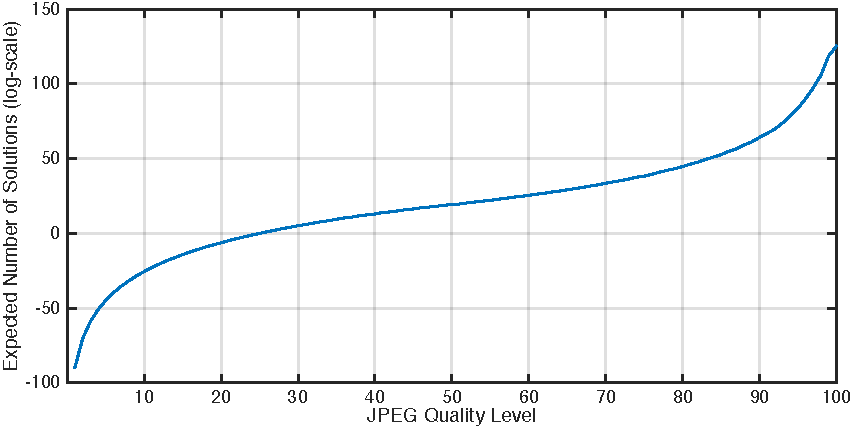
\includegraphics[width=0.8\textwidth]{figures/solcount2.pdf}\\[0em]
  \caption{Number of expected solutions}
  \label{fig:solution_count}
\end{figure}

We first tried applying CVC4, Yices, and Z3 to the problem by encoding the
problem in a format supported by the solver. We used SMT-LIB for CVC4 and Z3,
and Yices' native format for it. Unfortunately, none of these tools were able to
solve any of the problems at quality levels from $1$ to $100$ within a 1 hour
cutoff for each problem.  We also ran all three solvers without success
for over two months on problems at quality levels \(99\) and \(1\).

We have had much better success when BLT is applied to these problems.  In our
testing, BLT has been able to find solutions to all problems at quality level
\(27\) and higher.  BLT found that the problems at quality levels
\(1\) through \(18\) were \emph{unsatisfiable}. We include a chart of BLT's
runtime in Figure \ref{fig:blt-perf}. In the plot, solid points denote
problems for which BLT returns SAT, whereas $\times$ points denote problems
where BLT returns UNSAT. The large number of problems with roughly constant
runtime (mostly on the right side of the plot) have the property that the
Babai point (mentioned in section \ref{ssec:blt-optimizations}) is already a
solution and thus almost no search is needed. In the filled region between levels
19 and 26, BLT failed to terminate in the $1$ hour cutoff.

We should note that BLT is performing floating point arithmetic, and so when BLT
returns unsat there is a risk that floating point rounding error lead to BLT
detecting a branch was infeasible when it was in fact infeasible.  This may also
account for some of the performance gap, between BLT and the above solvers, but
we suspect it is unlikely that precision alone can account for the more than 6
orders of magnitude runtime difference we have observed above.

\begin{figure}[htb]
  \centering
    \includegraphics[width=0.8\textwidth]{figures/blt_benchmark.pdf}
    \caption{BLT Runtime vs. Problem Level}
    \label{fig:blt-perf}
\end{figure}

\FloatBarrier

%We have run the problem on other problems with varying constraints.
%These experiments have showna correlation between the number of expected
%solutions, and whether the solver will succeed at finding solutions.
%However, the correlation is not strict even on closely related problems.
%To illustrate this, we considered a second problem \(Q\) for which we
%added an additional row of constraints:
%
%\begin{verbatim}
%Q = { 'xx' 'xx' 'xx' 'xx' 'xx' 'xx' 'xx' 'xx'
%      'xx' '48' '65' '6c' '6c' '6f' '20' 'xx' % "Hello "
%      'xx' '57' '6f' '72' '6c' '64' '21' 'xx' % "World!"
%      'xx' 'xx' 'xx' 'xx' 'xx' 'xx' 'xx' 'xx'
%      'xx' 'xx' 'xx' 'xx' 'xx' 'xx' 'xx' 'xx'
%      'xx' '48' '65' '6c' '6c' '6f' '20' 'xx' % "Hello "
%      'xx' '57' '6f' '72' '6c' '64' '21' 'xx' % "World!"
%      'xx' 'xx' 'xx' 'xx' 'xx' 'xx' 'xx' 'xx' };
%\end{verbatim}
%
%Due to the additional rows of constraints, this problem has fewer
%solutions at a given quality level. In this case, BLT was able to find
%solutions for problems down to quality level \(68\), which was expected
%to have \(601\) solutions. In contrast, BLT was unable to solve the
%original problem \(P\) at quality level \(30\) even though that problem
%was expected to have just over \(10^{5}\) solutions. BLT was also able to
%show unsatisfiability for quality levels \(1\) through \(9\), showing
%that BLT is better able to show unsatisfiability on these problems.

%We plan to continue experiments to better understand the performance of
%BLT on different problems. Given that BLT relies on search and ILP is an
%NP-hard problem, we do not expect to be able to solve every problem, or
%even be able to accurately predict whether a particular problem can
%solved. However, research on random Boolean \(k\)-SAT problems has shown
%a clear relationships between problem satisfiability and the clause to
%variable ratio {[}3{]}. One may hope to establish similar relationships
%for bounded ILP problems.
